\documentclass[border=3pt]{standalone}
\usepackage[T1]{fontenc}
\usepackage{tikz}
\usetikzlibrary{shapes.geometric, arrows.meta, positioning}

\definecolor{stage1}{RGB}{66,133,244}
\definecolor{stage2}{RGB}{234,67,53}
\definecolor{stage3}{RGB}{251,188,4}
\definecolor{stage4}{RGB}{52,168,83}
\definecolor{boxbg}{RGB}{245,245,250}

\begin{document}
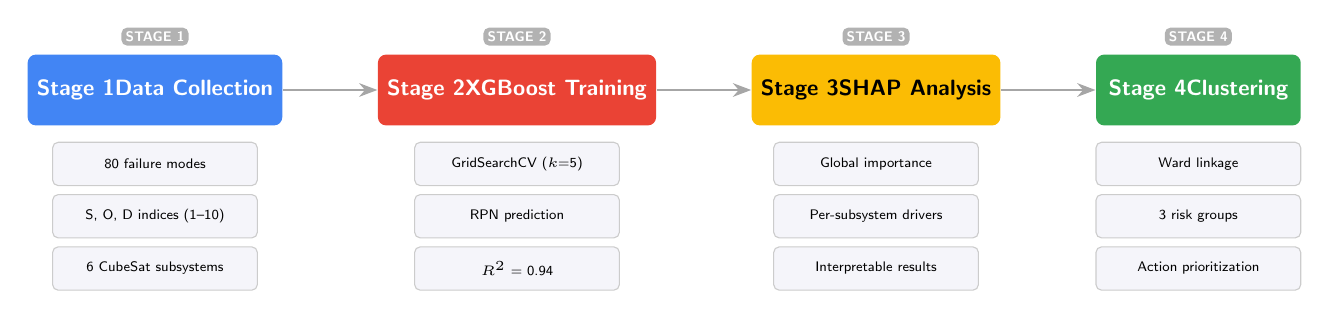
\begin{tikzpicture}[
    node distance=0.4cm and 0.6cm,
    >=Stealth,
    stage/.style={
        rectangle, rounded corners=3pt, minimum width=2.6cm, minimum height=0.9cm,
        text centered, font=\sffamily\footnotesize\bfseries, text=white
    },
    detail/.style={
        rectangle, rounded corners=2pt, minimum width=2.6cm, minimum height=0.55cm,
        text centered, font=\sffamily\tiny, fill=boxbg, draw=gray!40
    },
    arrow/.style={->, thick, color=gray!70},
    label/.style={font=\sffamily\tiny\bfseries, text=white, fill=gray!60, rounded corners=2pt, inner sep=1.5pt}
]

% Stage 1
\node[stage, fill=stage1] (s1) {Stage 1\\Data Collection};
\node[detail, below=0.2cm of s1] (d1a) {80 failure modes};
\node[detail, below=0.1cm of d1a] (d1b) {S, O, D indices (1--10)};
\node[detail, below=0.1cm of d1b] (d1c) {6 CubeSat subsystems};

% Stage 2
\node[stage, fill=stage2, right=1.2cm of s1] (s2) {Stage 2\\XGBoost Training};
\node[detail, below=0.2cm of s2] (d2a) {GridSearchCV ($k$=5)};
\node[detail, below=0.1cm of d2a] (d2b) {RPN prediction};
\node[detail, below=0.1cm of d2b] (d2c) {$R^2$ = 0.94};

% Stage 3
\node[stage, fill=stage3, text=black, right=1.2cm of s2] (s3) {Stage 3\\SHAP Analysis};
\node[detail, below=0.2cm of s3] (d3a) {Global importance};
\node[detail, below=0.1cm of d3a] (d3b) {Per-subsystem drivers};
\node[detail, below=0.1cm of d3b] (d3c) {Interpretable results};

% Stage 4
\node[stage, fill=stage4, right=1.2cm of s3] (s4) {Stage 4\\Clustering};
\node[detail, below=0.2cm of s4] (d4a) {Ward linkage};
\node[detail, below=0.1cm of d4a] (d4b) {3 risk groups};
\node[detail, below=0.1cm of d4b] (d4c) {Action prioritization};

% Arrows
\draw[arrow] (s1) -- (s2);
\draw[arrow] (s2) -- (s3);
\draw[arrow] (s3) -- (s4);

% Stage labels
\node[label, above=0.1cm of s1] {STAGE 1};
\node[label, above=0.1cm of s2] {STAGE 2};
\node[label, above=0.1cm of s3] {STAGE 3};
\node[label, above=0.1cm of s4] {STAGE 4};

\end{tikzpicture}
\end{document}
